\documentclass[final,hyperref={pdfpagelabels=false}]{beamer}
\usepackage{grffile}
\mode<presentation>{\usetheme{PosterLogProb}}
\usepackage[english]{babel}
\usepackage[latin1]{inputenc}
\usepackage{amsmath,amsthm, amssymb, latexsym}
\usepackage{epsfig}
\usepackage{listings}
\usepackage{lstlinebgrd}

\usepackage[orientation=portrait,size=a0,scale=1.4,debug]{beamerposter}
\providecommand\thispdfpagelabel[1]{}
\setbeamertemplate{bibliography entry title}{\color{black}}
\setbeamertemplate{bibliography entry location}{}
\setbeamertemplate{bibliography entry note}{}

\usepackage{array,booktabs,tabularx}
\newcolumntype{Z}{>{\centering\arraybackslash}X} % centered tabularx columns
\newcommand{\pphantom}{\textcolor{ta3aluminium}} % phantom introduces a vertical space in p formatted table columns??!!

\listfiles

\usepackage{amsthm}
%%%%%%%%%%%%%%%%%%%%%%%%%%%%%%%%%%%%%%%%%%%%%%%%%%%%%%%%%%%%%%%%%%%%%%%%%%%%%%%%%%%%%%


 \title{\huge\bfseries\hspace*{-1em} Empurrando Juntos: \\A platform for social participation}
\date{}
\author{\large Tallys Martins
\and Dylan Guedes
\and Luan Guimar�es \\
\and Ricardo Poppi
\and Henrique Parra
\and Paulo Meirelles
}
\institute[UNB/CD]{University of Bras�lia and Cidade Democr�tica NGO, Brazil}

\newlength{\columnheight}
\setlength{\columnheight}{105cm}


\begin{document}
\setbeamertemplate{caption}{\raggedright\insertcaption\par}
\begin{frame}
  \begin{columns}
    % ---------------------------------------------------------%
    % Set up a column
    \begin{column}{.49\textwidth}
      \begin{beamercolorbox}[center,wd=\textwidth]{postercolumn}
        \begin{minipage}[T]{.95\textwidth}
          \parbox[t][\columnheight]{\textwidth}{

\begin{block}{What is Empujando Juntos}

  \begin{itemize}
    \item A Free Open Source Software for social participation that aims to
    increase communication between majority and minority, blowing bubbles of
    opinion.

    \item A tool for opinion polls that allows activists and non extremist people
    to engage regular people in online discussions.

    \item Based on Polis, we deliver better experiences on debate process
    with the ``crowdsource`` participation concept, which fosters
    more engagement than standard models like forum/thread.
  \end{itemize}
\end{block}

\begin{block}{Why Empurrando Juntos?}
  \begin{itemize}
    \item Encourages the interaction between different groups of opinion, blowing
    bubbles of opinion and addressing the manipulation phenomenon of social media

    \item Brings new resources using gamification concepts based on the profiles
    of the participants as a mean to bring diversity to online discussions.

    \item 100\% FOSS.
  \end{itemize}
\end{block}

\begin{block}{Polis Features}
  \begin{itemize}
    \item Allow people to create online conversations to debate about any subject,
    anonymous or not.

    \item People can to give their opinion by simple clicking in ``agree``,
    ``disagree`` or ``skip`` in other's comments.

    \item Identify different groups of opinion based on the reactions of the
    participants in the comments using clustering algorithms.

    \item Identify majority and minority consensus in the global scope and in
    each group scope. 
  \end{itemize}
\end{block}

\begin{block}{Empujando Juntos Features}
  \begin{itemize}
    \item Uses Polis engine to obtain the groups of opinion.

    \item Mobile responsive and minimalist design on top of Polis embed iframe.

    \item Provides a resource that we called ``the Push``. People in ownership of
    this ability (gamification) are able to send direct messages and create events in the platform.

    \item The ``Push`` is given to special actors in the groups formed by Polis.
    Three profiles are considered, the activist, the bridge and the consultation
    owner.

    \begin{figure}
      \begin{center}
        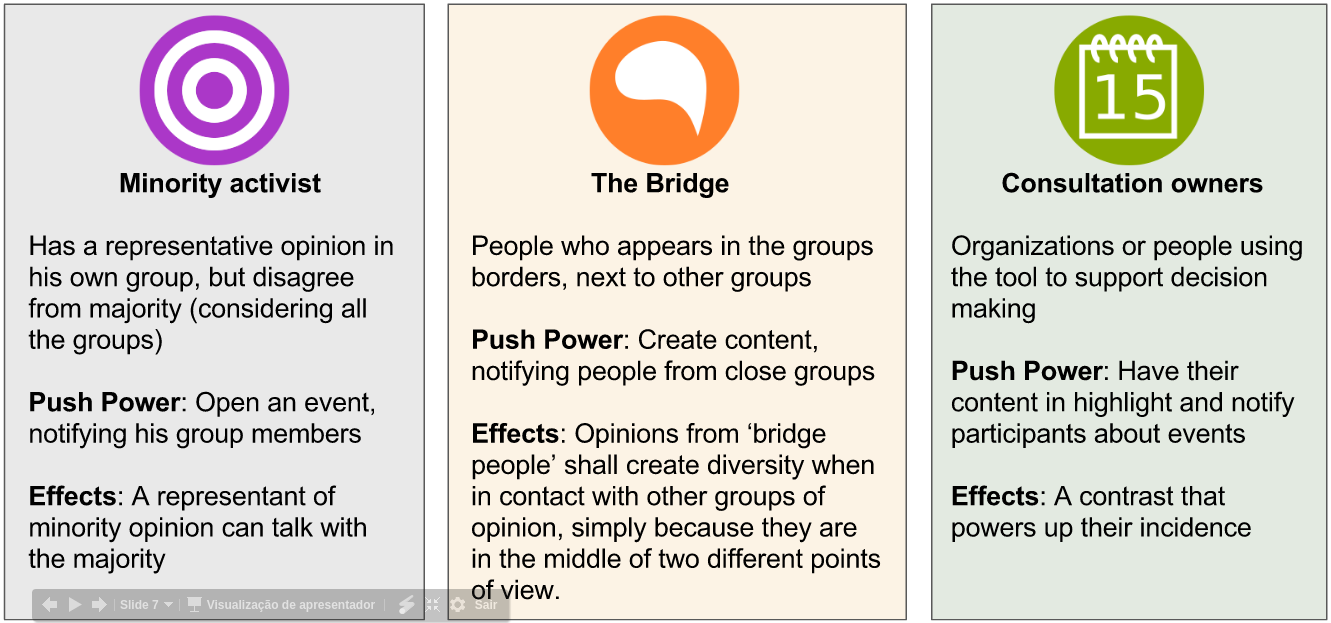
\includegraphics[scale=1.3]{../images/userprofiles.png}
        \caption{Profiles identified by Empurrando Juntos}
        \label{fig:background:free-software-repository}
      \end{center}
    \end{figure}
  
    \item Monitoring Polis conversations created through the App
    to identify activists and bridge participants to give them the ``Push``
    power.

    \item Activists can open events and notify people in his group cluster.

    \item Comments created by bridge people are spread to others by direct
    notifications.

    \item Consultation creators have their content highlighted and can also open
    events in the platform, like activists
  \end{itemize}
\end{block}

%-------------------------------------------------------------------------------
}
\end{minipage}
\end{beamercolorbox}
\end{column}
% ---------------------------------------------------------%
% end the column

% ---------------------------------------------------------%
% Set up a column
\begin{column}{.49\textwidth}
  \begin{beamercolorbox}[center,wd=\textwidth]{postercolumn}
    \begin{minipage}[T]{.95\textwidth} % tweaks the width, makes a new \textwidth
      \parbox[t][\columnheight]{\textwidth}{ % must be some better way to set the the height, width and textwidth simultaneously

\begin{block}{System Architecture}
	\begin{itemize}
    \item Front-end application, written in React Native 
    and a NodeJS server.

    \item The server module is responsible for managing users, ``the Push'', and
    to make the interface with Polis API
  \end{itemize}

  \begin{figure}
    \begin{center}
      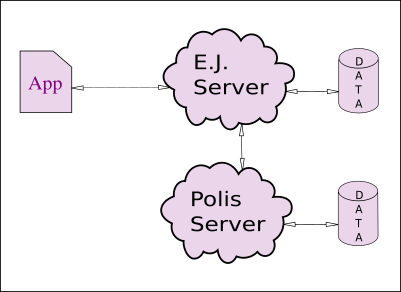
\includegraphics[scale=1.5]{../images/architecture-1.png}
      \caption{Simplified architecture of the system}
      \label{fig:architecture}
    \end{center}
  \end{figure}
\end{block}

\begin{block}{Integration with Polis}

\end{block}

\begin{block}{Final Remarks}
  \begin{itemize}
    \item Pushing Together arise as a potential tool to bridge dialog between society and
    the state, making different analyzes about the opinion of the distinct groups
    and also opening new possibilities for the expression of these opinions with ``the
    Push`` resource. Besides, the project was born with transparency and collaboration
    principles, building a base for a prospective evolution.

    \item We are now working on a research to evolve the clustering service that
    will fit our application model. Parallelly, our next steps include evolving the
    mobile application using mocked data and validating the user interface.

    \item All our contributions are published in open repositories available at:
      \begin{itemize}
        \item \url{github.com/cidadedemocratica/pushingtogether}
        \item \url{github.com/cidadedemocratica/app_pushingtogether}
      \end{itemize}
  \end{itemize}
\end{block}
      }
        \end{minipage}
      \end{beamercolorbox}
    \end{column}
  \end{columns}
\end{frame}
\end{document}
